%\documentclass[12pt]{article}
\documentclass[aip,jcp,preprint,superscriptaddress,floatfix]{revtex4-1}
\usepackage{url,graphicx,tabularx,array,geometry,amsmath,listings}
\setlength{\parskip}{2ex} %--skip lines between paragraphs
\setlength{\parindent}{20pt} %--don't indent paragraphs

\usepackage[colorinlistoftodos,prependcaption,textsize=tiny]{todonotes} %--TODO notes

\setlength{\headheight}{-50pt}
\setlength{\textheight}{700pt}
\setlength{\textwidth}{500pt}
\setlength{\oddsidemargin}{-10pt}
\setlength{\footskip}{50pt}
\usepackage{graphicx}% Include figure files
\usepackage{bm}
\usepackage{hyperref}
\usepackage{amssymb}
\usepackage{amsmath}
\graphicspath{{./Figures/}}

%-- Commands for header
\renewcommand{\title}[1]{\textbf{\large{#1}}\\}
\renewcommand{\line}{\begin{tabularx}{\textwidth}{X>{\raggedleft}X}\hline\\\end{tabularx}\\[-0.5cm]}
\newcommand{\leftright}[2]{\begin{tabularx}{\textwidth}{X>{\raggedleft}X}#1%
& #2\\\end{tabularx}\\[-1cm]}

%-- Convenient shortcuts
\newcommand{\x}{\mathbf{x}}
\newcommand{\vel}{\mathbf{v}}
\newcommand{\splitting}[1]{{\bf \sf #1}} %%% O, V, R symbols and splittings
\newcommand{\dt}{{\differential t}} % infinitesimal
\newcommand{\differential}{\mathrm{d}} % differential
\newcommand{\substep}{h} % partial timestep

%\linespread{2} %-- Uncomment for Double Space
\begin{document}

\title{\center{Molecular Dynamics} }
\rule{\textwidth}{1pt}
\leftright{The Molecular Sciences Software Institute}{Eliseo Marin-Rimoldi and John D.~Chodera} %-- left and right positions in the header

\bigskip

\section{Introduction}

Your first assignment consisted on implementing a Monte Carlo (MC) simulation
for the Lennard-Jones (LJ) particle in the canonical ensemble. 
As part of this task, you developed code that computed pair-wise energies and forces for this model, 
as well as functions that computed interaction energies between molecules,
the total system potential energy, and the atomic virial for the estimation of pressure.

The objective of the new task is to extend your code by including the
necessary functionality to simulate the NVT ensemble of configurations 
of the LJ model using the molecular dynamics (MD). You will be 
assigned to work in teams to develop this project. The team will
decide how is best to design the new code: What functionality should be shared
between the two methods? What should the library should look like? How can
we improve reusability and extensibility? What data
structures should be used? Which unit tests should be implemented?
The primary learning goal of this activity is to think about interoperability and teamwork.

In the following sections, we illustrate how to implement a Langevin integrator to sample from the NVT ensemble, where our primary focus will be on expectations of configurational properties.

\subsection{Molecular dynamics (MD) and Langevin integrators}

Molecular dynamics (MD) is a highly popular technique to simulate both equilibrium and nonequilibrium properties of molecular systems.
Here, we focus on the estimation of equilibrium configurational properties $\left< Q \right>$ of isothermal (NVT) systems at fixed volume.
While the MC scheme we implemented earlier is a simple and practical way to estimate configurational properties in simple systems, in more complex systems, it becomes difficult to construct moves that have high acceptance rates because couplings between various degrees of freedom become more complex and nonlinear.
Molecular dynamics can circumvent these problems by allowing the instantaneous \emph{forces} to help guide sampling of configuration space, which can follow highly nonlinear regions of high probability---at the expense of requiring potentially many timesteps in order to generate effectively uncorrelated samples from the target equilibrium probability density.
If a high-quality integrator that preserves dynamical properties is also used, we can also get additional dynamical properties inaccessible in Monte Carlo simulation, such time-correlation functions, transition rates, and viscosities. 

Langevin integrators are widely employed to numerically simulate the equilibrium thermodynamics and kinetics of microscopic molecular systems.
The origin of these integrators lies in the \emph{memoryless Langevin equation}~\cite{langevin:1908:langevin-dynamics}, which describes the behavior of condensed phase systems subject to random weak collisions with fictitious bath particles at thermal equilibrium,
\begin{equation}
d \begin{bmatrix} \x\\ \vel \end{bmatrix} =
\underbrace{\begin{bmatrix} \vel \\ 0 \end{bmatrix}}_\splitting{R} \dt +
\underbrace{\begin{bmatrix} 0 \\ - M^{-1} \nabla U(\x) \end{bmatrix}}_\splitting{V} \dt +
\underbrace{\begin{bmatrix} 0 \\ - \gamma \vel \dt + \sigma M^{1/2} d W \end{bmatrix}}_\splitting{O}
\label{equation.LangevinEquation}
\end{equation}
Here $\x$ and $\vel$ denote the positions and velocities of all particles in the system, $t$ is time, and $M$ the diagonal mass matrix. 
The constant $\sigma^2 = (2 k_B T \, \gamma)$ quantifies the rate of heat exchange with the bath, with $k_B T$ denoting the thermal energy and $\gamma$ the collision rate (with dimensions of inverse time), and $W(t)$ is a standard multidimensional Wiener process~\cite{LeimkuhlerMatthewsBook,LelievreBook}.

While this equation in principle has an exact solution to update the positions $\x$ and velocities $\vel$ by a timestep $\Delta t$, 
\begin{eqnarray}
\rho(\x, \vel; t + \Delta t) &=& e^{- \mathcal{L} \Delta t} \rho(\x, \vel; t) = e^{- (\mathcal{L}_\splitting{R} + \mathcal{L}_\splitting{V} + \mathcal{L}_\splitting{O}) \Delta t} \rho(\x, \vel; t)
\end{eqnarray}
we cannot integrate the whole equation analytically.
Instead, we can take the time-evolution operator $\mathcal{L}$ that corresponds to the action of Eq.~\ref{equation.LangevinEquation} applied to a probability density and factor it into an \emph{approximate} symmetric product of operators corresponding to parts of Eq.~\ref{equation.LangevinEquation} that can be analytically integrated, forming a variety of integrators:
\begin{eqnarray}
e^{- \mathcal{L} \Delta t} &\approx& \\
&\approx& e^{-\mathcal{L}_\splitting{O V R V O} \Delta t} = e^{-\mathcal{L}_\splitting{O} \frac{\Delta t}{2}} e^{-\mathcal{L}_\splitting{V} \frac{\Delta t}{2}} e^{-\mathcal{L}_\splitting{R} \Delta t} e^{-\mathcal{L}_\splitting{V} \frac{\Delta t}{2}} e^{-\mathcal{L}_\splitting{O} \frac{\Delta t}{2}} \\
&\approx& e^{-\mathcal{L}_\splitting{V R O R V} \Delta t} = e^{-\mathcal{L}_\splitting{V} \frac{\Delta t}{2}} e^{-\mathcal{L}_\splitting{R} \frac{\Delta t}{2}} e^{-\mathcal{L}_\splitting{O} \Delta t} e^{-\mathcal{L}_\splitting{R} \frac{\Delta t}{2}} e^{-\mathcal{L}_\splitting{V} \frac{\Delta t}{2}} \\
\end{eqnarray}
These symmetric splittings are called Trotter splittings, and they possess good numerical properties that have been analyzed in detail~\cite{LeimkuhlerMatthewsBook,LelievreBook}.

The action of these individual operators can be analytically expressed:
\begin{eqnarray}
\splitting{R} \:\: : \:\: \begin{bmatrix} \Delta\x\\ \Delta\vel \end{bmatrix} =
\color{black} \underbrace{\begin{bmatrix} \vel \\ 0 \end{bmatrix}}_\splitting{R} \substep \color{black}
\color{white} + \underbrace{\begin{bmatrix} 0 \\ - M^{-1} \nabla U(\x) \end{bmatrix}}_\splitting{V} \substep \color{black}
\color{white} + \underbrace{\begin{bmatrix} 0 \\ (a_{h} - 1) \vel + b_{h} \sqrt{k_B T / m} \xi \end{bmatrix}}_\splitting{O} \color{black} \\
\splitting{V} \:\: : \:\: \begin{bmatrix} \Delta\x\\ \Delta\vel \end{bmatrix} =
\color{white} \underbrace{\begin{bmatrix} \vel \\ 0 \end{bmatrix}}_\splitting{R} \substep \color{black}
\color{black} + \underbrace{\begin{bmatrix} 0 \\ - m^{-1} \nabla U(\x) \end{bmatrix}}_\splitting{V} \substep \color{black}
\color{white} + \underbrace{\begin{bmatrix} 0 \\ (a_{h} - 1) \vel + b_{h} \sqrt{k_B T / m} \xi \end{bmatrix}}_\splitting{O} \color{black} \\
\splitting{O} \:\: : \:\: \begin{bmatrix} \Delta\x\\ \Delta\vel \end{bmatrix} =
\color{white} \underbrace{\begin{bmatrix} \vel \\ 0 \end{bmatrix}}_\splitting{R} \substep \color{black}
\color{white} + \underbrace{\begin{bmatrix} 0 \\ - M^{-1} \nabla U(\x) \end{bmatrix}}_\splitting{V} \substep \color{black}
\color{black} + \underbrace{\begin{bmatrix} 0 \\ (a_{h} - 1) \vel + b_{h} \sqrt{\frac{k_B T}{m}} \xi \end{bmatrix}}_\splitting{O} \color{black}
\end{eqnarray}
where $h$ is the time interval over which the integrator is applied (either $\Delta t$ or $\Delta t / 2$) for this substep, $a_h \equiv e^{-\gamma h}$, and $b_h = \sqrt{1 - a_h^2}$, and $\xi \sim \mathcal{N}(0,1)$ is a standard normal variate.
You will recognize $-m^{-1} \nabla U$ as the instantaneous acceleration.

Putting this together, we can construct two useful concrete Langevin integrators from these components which possess very different properties (Figure~\ref{figure:timestep-dependent-error}):

\subsection{\splitting{OVRVO}}

The \splitting{OVRVO} integrator (also known as VVVR~\cite{VVVR} or the integrator of Bussi and Parrinello~\cite{BussiParrinello}) is likely to be most familiar as the core of the integrator is equivalent to the incredibly popular velocity Verlet integrator of Swope et.~al~\cite{VelocityVerlet}:

\begin{eqnarray}
\vel_{t+1/4} &=& e^{-\gamma \Delta t / 2} \vel_t + \sqrt{1 - e^{-\gamma \Delta t}} \sqrt{\frac{k_B T}{m}} \xi_{t+1/4} \nonumber \\
\vel_{t+1/2} &=& \vel_{t+1/4} +  \frac{\Delta t}{2} m^{-1} f(\x_t) \nonumber \\
\x_{t+1} &=& \x_t + \Delta t \, \vel_{t+1/2} \nonumber \\
\vel_{t+3/4} &=& \vel_{t+1/2} +  \frac{\Delta t}{2} m^{-1} f(\x_{t+1}) \nonumber \\
\vel_{t+1} &=& e^{-\gamma \Delta t / 2} \vel_{t+3/4} + \sqrt{1 - e^{-\gamma \Delta t}} \sqrt{\frac{k_B T}{m}} \xi_{t+3/4} 
\end{eqnarray}
The fractional sub-timesteps are simply intermediate values that are convenient for both writing and implementing the integrator.
The stochastic variables $\xi_{t+1/4}, \xi_{t+3/4} \sim \mathcal{N}(0,1)$ are standard normal random variates (of the sort generated by \href{https://docs.scipy.org/doc/numpy/reference/generated/numpy.random.randn.html}{\tt numpy.random.randn}) and a separate random variable must be used for each degree of freedom for each particle and for each instance of $\xi$.

\subsection{\splitting{VRORV}}
The \splitting{VRORV} integrator (also known as the BAOAB integrator by Leimkuhler and Matthews~\cite{gBAOAB,BAOAB}) will be less familiar, but it possesses superior accuracy for configurational properties, so we will make use of it here:
\begin{eqnarray}
\vel_{t+1/4} &=& \vel_{t} +  \frac{\Delta t}{2} m^{-1} f(\x_t) \nonumber \\
\x_{t+1/2} &=& \x_t + \frac{\Delta t}{2} \vel_{t+1/4} \nonumber \\
\vel_{t+3/4} &=& e^{-\gamma \Delta t} \vel_{t+1/4} + \sqrt{1 - e^{-2 \gamma \Delta t}} \sqrt{\frac{k_B T}{m}} \xi_{t+1/2} \nonumber \\
\x_{t+1} &=& \x_{t+1/2} + \frac{\Delta t}{2} \vel_{t+3/4} \nonumber \\
\vel_{t+1} &=& \vel_{t+3/4} +  \frac{\Delta t}{2} m^{-1} f(\x_{t+1}) \nonumber \\
\end{eqnarray}

\subsection{Forces and switching functions}

Unlike Monte Carlo methods, molecular dynamics integrators require both the the potential energies and forces to be everywhere continuous in order to produce well-behaved dynamics and sampling.
Because the potential function you implemented for Monte Carlo simply used a cutoff, this requires we add an additional option to use a switching function to ensure force continuity:
\begin{eqnarray}
U_\mathrm{sw}(r) = U_{LJ}(r) \, S(r)
\end{eqnarray}
where $U_{LJ}(r)$ is the Lennard-Jones potential you implemented earlier, 
\begin{equation}
U(r) = 4 \epsilon \left[\left(\frac{\sigma}{r}\right)^{12} -\left(\frac{\sigma}{r}\right)^{6} \right] 
\end{equation}
and the switching function $S(r)$ is selected to have a value of unity for $r \in [0, r_\mathrm{sw}]$, smoothly interpolates between 1 and 0 for $r \in (r_\mathrm{sw}, r_\mathrm{cut})$, and is zero for $r \in [r_\mathrm{cut}, \infty)$, with continuous first and second derivatives everywhere.
One such switching function come from Steinbach and Brooks~\cite{SwitchingFunction,Shirts.JCP.119.5740.2003}:
\begin{eqnarray}
S(r) &=& \begin{cases}
1 & r \le r_\mathrm{sw} \\
\frac{(r_\mathrm{cut}^2 - r^2)^2 (r_\mathrm{cut}^2 + 2 r^2 - 3 r_\mathrm{sw}^2)}{(r_\mathrm{cut}^2 - r_\mathrm{sw}^2)^3} & r_\mathrm{sw} < r < r_\mathrm{cut} \\
0 & r \ge r_\mathrm{cut}
\end{cases}
\end{eqnarray}
To compute the force on atom $i$, we use the chain rule:
\begin{eqnarray}
f_k(\textbf{r}^N) &=& - \nabla_{\textbf{r}_k} \sum_{i < j} U(r_{ij}) =  - \sum_{i < j} \nabla_{\textbf{r}_k} \left[ U_{LJ}(r_{ij}) \, S(r_{ij}) \right] \nonumber \\
&=& - \sum_{i \ne k} \left\{ [ \nabla_{\textbf{r}_k} U_{LJ}(r_{ik}) ] \, S(r_{ik}) + U_{LJ}(r_{ik}) \,  \nabla_{\textbf{r}_k} S(r_{ik}) \right\}
\end{eqnarray}
The component derivatives are simply given by
\begin{eqnarray}
\nabla_{\mathbf{r}_k} U_{LJ}(r_{ik}) &=& \left. \frac{\partial U_{LJ}(r)}{\partial r} \right|_{r_{ik}} \nabla_{\mathbf{r}_k} r_{ik}  \\
&=& 4 \epsilon \left[- 12 \sigma^{12} r_{ik}^{-13} + 6 \sigma^6 r_{ik}^{-7} \right] \nabla_{\mathbf{r}_k} || \mathbf{r}_k - \mathbf{r}_i ||_2  \\
&=& - \frac{48 \epsilon}{r_{ik}} \left[2 \left(\frac{\sigma}{r}\right)^{12} - \left(\frac{\sigma}{r}\right)^{6} \right] \left[ \frac{\mathbf{r}_k - \mathbf{r}_i}{r_{ik}} \right]
\end{eqnarray}
and
\begin{eqnarray}
\nabla_{\mathbf{r}_k} S(r_{ik}) &=& \left. \frac{\partial S(r)}{\partial r} \right|_{r_{ik}} \nabla_{\mathbf{r}_k} r_{ik}  \\
&=&\frac{(12 r_{ik}) (r_{ik}^2 - r_\mathrm{cut}^2) (r_{ik}^2 - r_\mathrm{sw}^2)}{(r_\mathrm{cut}^2 - r_\mathrm{sw}^2)^3} \left[ \frac{\mathbf{r}_k - \mathbf{r}_i}{r_{ik}} \right] \\
\end{eqnarray}

\subsection{Technical considerations}

%\textbf{Energy conservation. } The velocity verlet algorithm has very good
%energy conservation properties. It is always a good check to see if 
%there is no drift in energy during the course of the simulation.

\textbf{Choice of timestep.} 
Unlike Metropolis Monte Carlo, molecular dynamics methods do not sample exactly from the target equilibrium density $\pi(\x,\vel)$, but instead sample from a density $\rho_{\Delta t}(\x,\vel)$ that increasingly deviates from the target equilibrium density as the timestep $\Delta t$ increases (Figure~\ref{figure:timestep-dependent-error}).
Using a timestep that is too large will result in large errors in the sampled density $\rho_{\Delta t}(\x)$ or, worse yet, unstable dynamics that might cause the simulation to ``explode''  and rapidly accumulate NaNs.

Traditional guidelines suggest restricting your timestep to be no bigger than $\frac{1}{10}$ the fastest vibrational frequency in the system.
For a pair of Lennard-Jones particles separated by $r_\mathrm{min} = 2^{1/6} \sigma$ where their interaction is minimized, the vibrational period for small oscillations about the minimum is given by
\begin{eqnarray}
T &\approx& 2 \pi \sqrt{ \frac{\mu}{K} } 
\end{eqnarray}
Here, the effective spring constant $K = \left. \frac{\partial^2 U_{LJ}}{\partial r^2} \right|_{r_\mathrm{min}} = 72 \epsilon / r_\mathrm{min}^2$ and the effective mass $\mu = (m^{-1} + m^{-1})^{-1} = m/2$ give a period of 
\begin{eqnarray}
T \approx 2 \pi \sqrt{\frac{2^{1/3} m \sigma^2}{144 \epsilon}} \approx 0.09354 \sqrt{\frac{m \sigma^2}{\epsilon}}
\end{eqnarray}
suggesting we should use a maximum timestep of $\Delta t \le T/10$.
More detailed discussion of the timestep-induced error can be found in Leimkuhler and Matthews~\cite{LeimkuhlerMatthewsBook} and work that uses nonequilibrium approaches to quantify this error~\cite{VVVR}.

\begin{figure}[h]
\centering
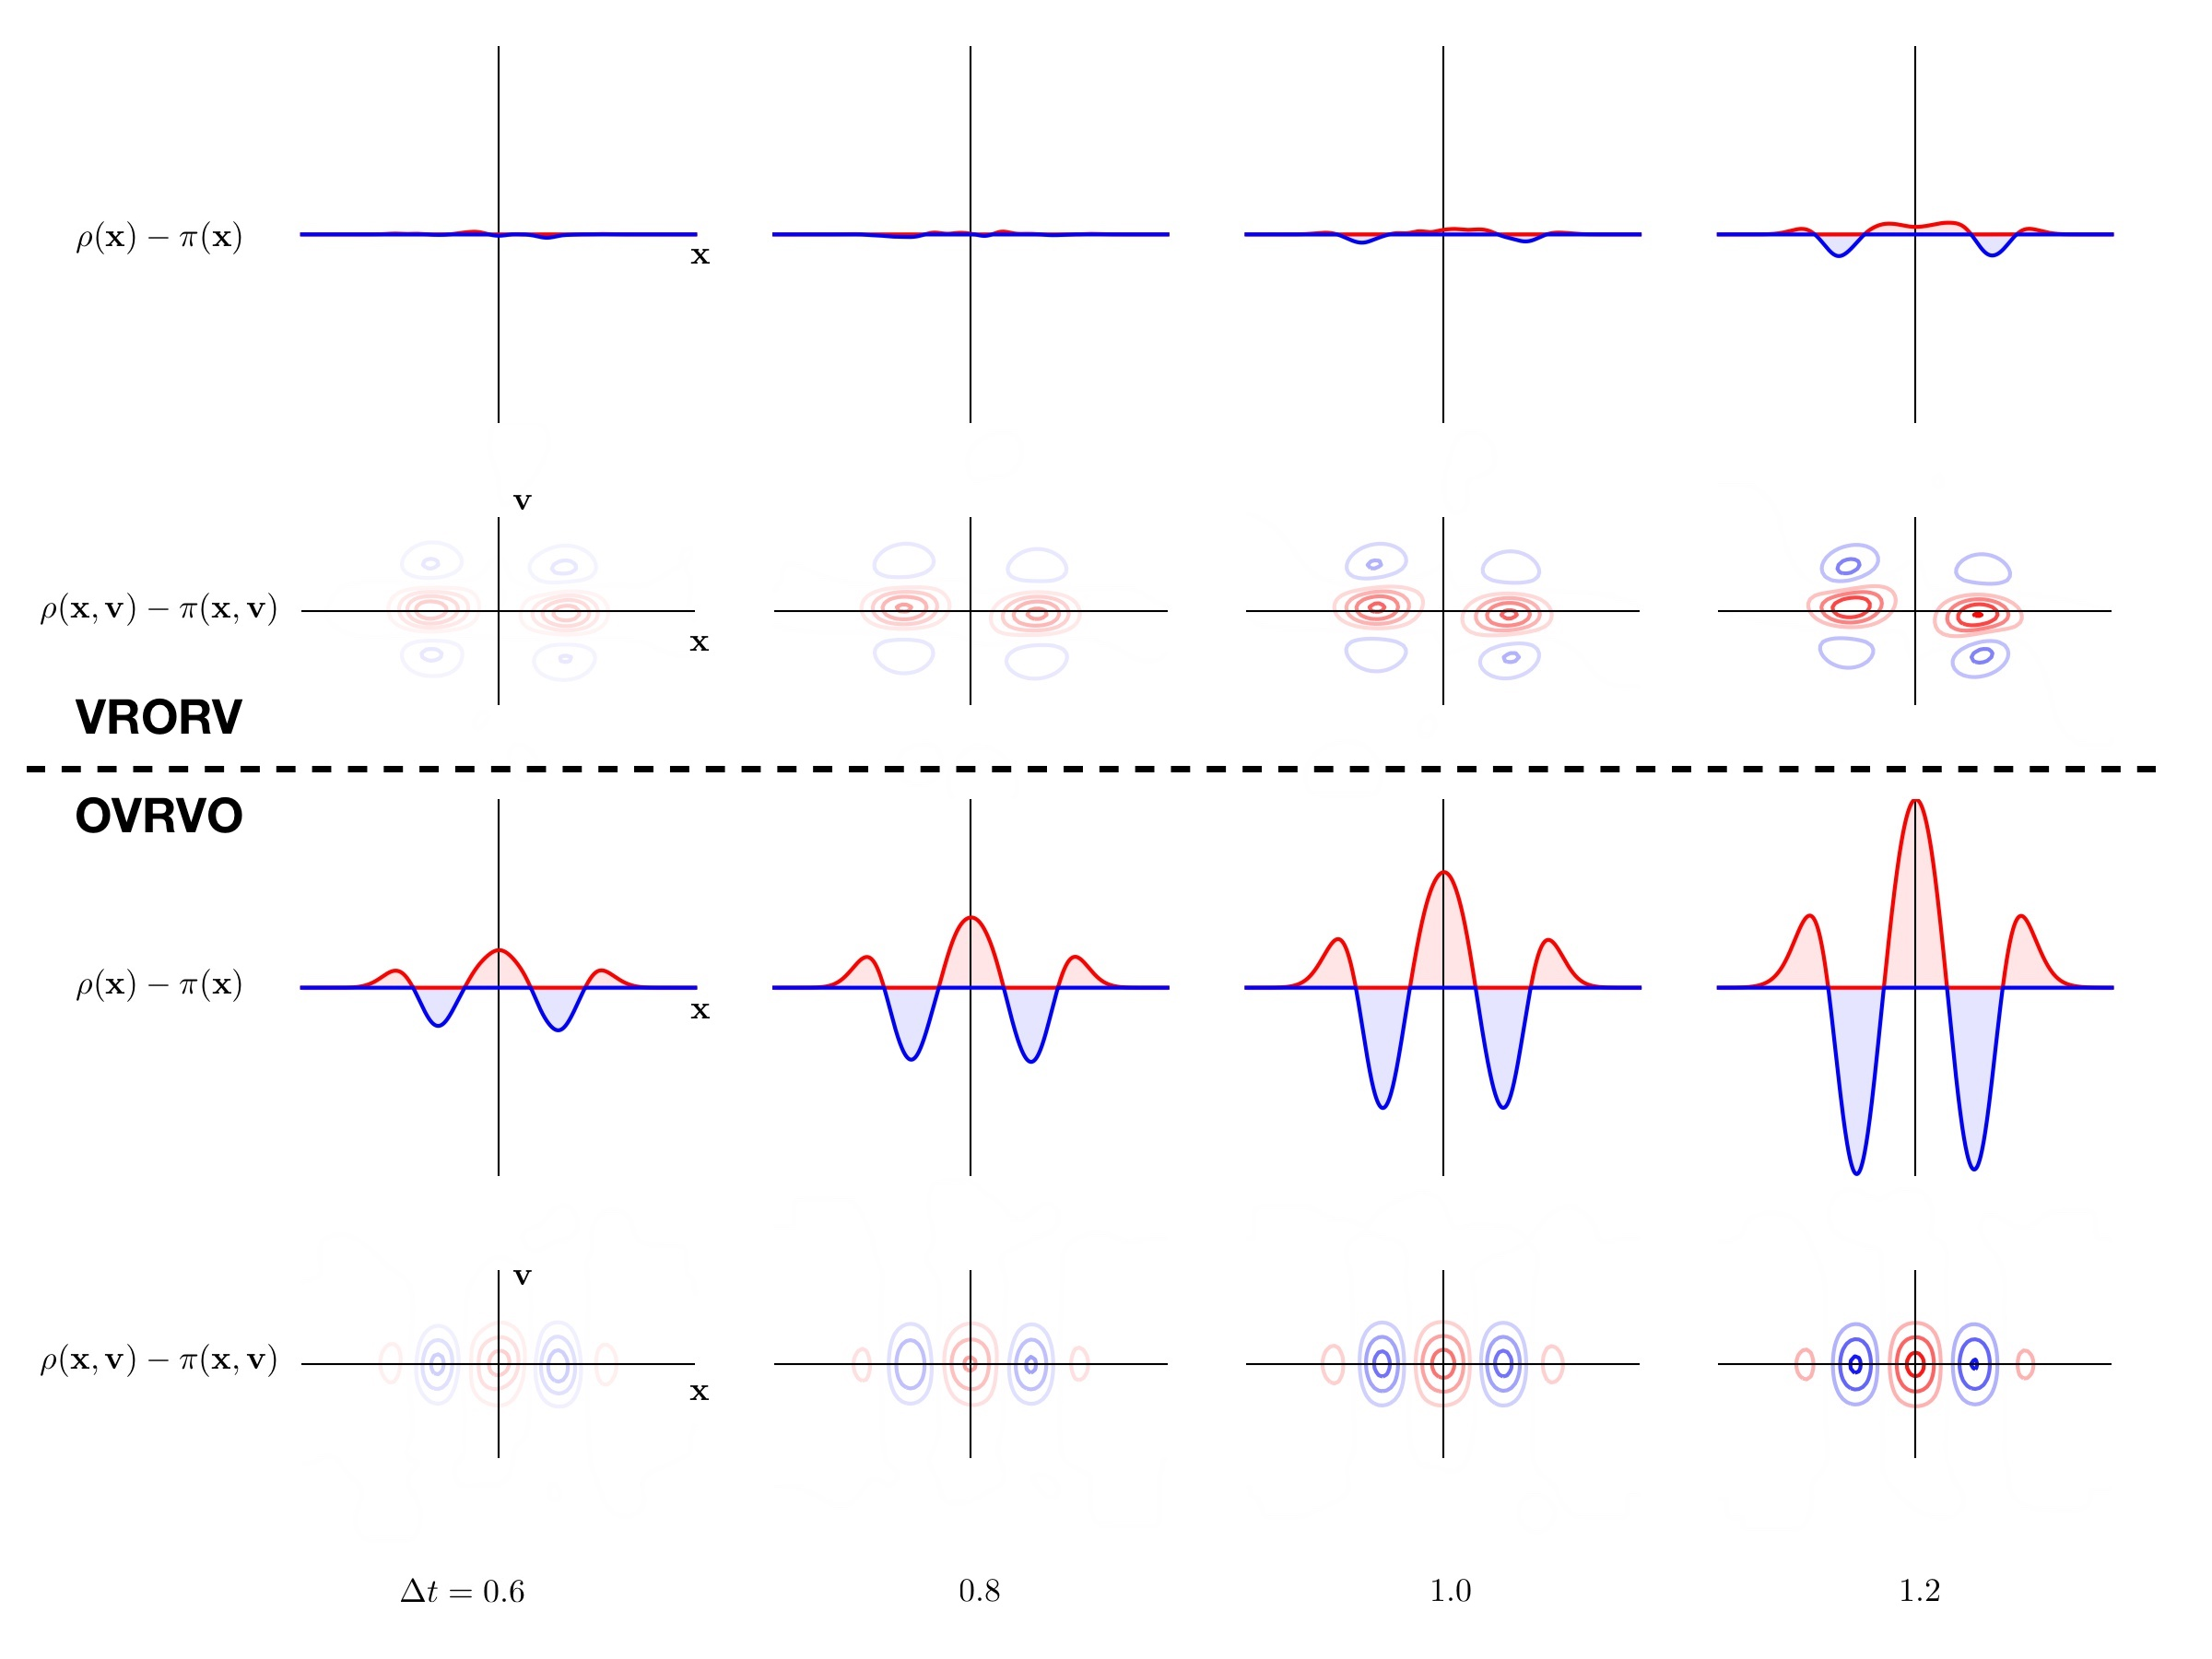
\includegraphics[width=1.0\textwidth]{figures/quartic_eq_joint_dist_array_w_x_marginals.jpg}

\caption{{\bf Different Langevin integrator splittings lead to different timestep-dependent errors in the sampled configuration and phase space densities.}
The quantity $\rho(\x,\vel) - \pi(\x,\vel)$ measures the deviation of the sampled phase space density $\rho_{\Delta t}(\x,\vel)$ from the target equilibrium density $\pi(\x,\vel)$ as a function of timestep for a quartic potential $U(x) = x^4$.
The marginal error in configuration space only, $\rho(\x) - \pi(\x)$, is the one-dimensional projection of this error.
Two different Langevin integrators derived from different Trotter splittings are shown: \splitting{VRORV} (also known as the BAOAB integrator by Leimkuhler and Matthews~\cite{gBAOAB,BAOAB}) and \splitting{OVRVO} (also known as VVVR~\cite{VVVR} or the integrator of Bussi and Parrinello~\cite{BussiParrinello}).
Integrators based on different splittings can lead to very different error properties in positions and velocities.
We recommend using VRORV if accurate sampling configurations is necessary (e.g.~for computing configurational properties) and OVRVO if accurate sampling of velocities is necessary (e.g.~for velocity correlation functions or kinetic properties).
\label{figure:timestep-dependent-error}
}
\end{figure}  

\textbf{Choice of collision rate $\gamma$.}
The Langevin integrator collision rate $\gamma$ has three different regimes:
\begin{itemize}
\setlength{\itemsep}{0em} %--don't put a huge amount of space between items in a list
\item If $\gamma = 0$, standard Newtonian dynamics is recovered, and no thermal control is applied. This is sometimes a good way to check that the code is working correctly, though energy is never conserved exactly due to the use of a finite-timestep.
\item If $\gamma$ is small ($\gamma \ll 1/\Delta t$), the dynamics is \emph{underdamped}. This is good for ensuring some thermal control while not hindering diffusion through phase space.
\item If $\gamma$ is large ($\gamma \gtrapprox 1/\Delta t$), the dynamics is \emph{overdamped}. Velocities will decorrelate very rapidly, and the system will behave in a very Brownian fashion. This is useful for initial equilibration if large initial forces would initially cause rapid heating in the underdamped limit.
\end{itemize}
For this exercise, we suggest using a collision in the underdamped limit, such as $\gamma \sim (500 \Delta t)^{-1}$.
 
\textbf{Initial positions.} 
For molecular dynamics simulations, the main consideration is that the initial forces must not be so large that the system rapidly heats up and becomes numerically unstable.
Standard biomolecular systems must generally be subjected to energy minimization to produce forces small enough to run molecular dynamics, but several options are available for the simple Lennard-Jones system considered here.
While placing atoms randomly is more dangerous as core overlaps might exist, leading to huge repulsion forces, as in the Monte Carlo example, it is possible to use a crystalline lattice as an initial configuration, since this configuration will generally have relatively small forces. 
You could even first relax the system using the translation moves of your MC code, which only use energy differences forces for sampling and hence will not become numerically unstable due to large forces; a sampled configuration generated from your MC code could be used to initialize dynamics.

\textbf{Initial velocities.} 
Initial velocities can be generated from the Maxwell-Boltzmann distribution at the desired temperature
\begin{equation}
	\rho \left(\mathbf{v}_i\right) = \left( \frac{m_i}{2 \pi k_B T} \right)^{1/2} \exp \left[ - \frac{m_i \mathbf{v}_i^2 } {2 k_B T }  \right]
\end{equation}
This can be done by sampling the velocities for each particle from a Gaussian distribution
\begin{equation}
       \mathbf{v}_i \sim \mathcal{N}(0, \sigma_i^2)
\end{equation}
where the variance $\sigma_i^2$ is given by
\begin{equation}
	\sigma_v^2 = \frac{k_B T}{m_i}
\end{equation}

% JDC: We don't need to remove COM translational velocities for Langevin integrators.
%Once the velocities are assigned to the atoms, we must set the system momentum to zero to avoid any translational drift. 
%We do this by 
%\begin{itemize}
%	\item Find the net momentum of the system $\mathbf{P} = \sum m_i \mathbf{v}_i$
%	\item Reassign initial atomic velocities as
%		\begin{equation}
%			\mathbf{v}_i \leftarrow \mathbf{v}_i - \frac{\mathbf{P}} { N m_i}
%		\end{equation}
%\end{itemize}

\textbf{Long-range dispersion correction.}
Because a switch function is now employed, we must use a modified form of the long-range dispersion correction that accounts for the switching off of the potential over $r \in [r_\mathrm{sw}, r_\mathrm{cut}]$.
The simplest way to implement this is to numerically compute the long-range correction via
\begin{eqnarray}
U_\mathrm{tail,sw} &=& N \frac{N}{V} \int_{r_\mathrm{sw}}^\infty 4 \pi r^2 \, dr \, U_{LJ}(r) [1 - S(r)]  \\
&=& U_\mathrm{tail,cut} + \frac{N^2}{V} \int_{r_\mathrm{sw}}^{r_\mathrm{cut}} 4 \pi r^2 \, dr \, U_{LJ}(r) [1 - S(r)] 
\end{eqnarray}
where the integral is performed using numerical quadrature, such as the \href{https://docs.scipy.org/doc/scipy/reference/generated/scipy.integrate.quad.html}{\tt scipy.integrate.quad}, and $U_\mathrm{tail,cut}$ is the cutoff-based long-range correction implemented for the MC code.

\textbf{Periodic boundary conditions and minimum image distance.} 
As in the MC case, your MD code should also implement these features.

\textbf{Temperature. } The instantaneous temperature in a simulation can be computed as 
\begin{equation}
	T = \frac{2 K}{N_{DOF} k_B}
\end{equation}

\subsection{Concrete tasks}

\begin{enumerate}
\setlength{\itemsep}{0em} %--don't put a huge amount of space between items in a list
\item \textbf{Extend potential and force computation to support the switching function.}
You will want to implement appropriate tests, but the choice of which tests are appropriate is up to you.
One important feature you may want to test is the consistency between the potential and force, since this is essential to obtaining correct results for molecular dynamics simulations; this may utilize numerical tests of derivatives obtained via finite-difference or automatic differentiation schemes such as \href{https://github.com/HIPS/autograd}{\tt autograd}.

\item \textbf{Implement the integrator and a simulation driver harness.}
You will want to implement the integrator and appropriate tests, as well as a small example program that lets you run a simple system and compute averages.

\item \textbf{Compute expectations of the reduced potential energy and pressure of a Lennard-Jones fluid at $N=500$, $T^*= 0.90$, $\rho^* = 0.001$ and $0.9$, $r_c = 3\sigma$.}
You can compare these results to your Monte Carlo code.

\item \textbf{Stretch goal: Implement a Monte Carlo barostat.}
A Monte Carlo barostat is a simple way to implement pressure control and can be used with both your MC and MD codes.
The move proceeds in a similar fashion to the Metropolis Monte Carlo algorithm for perturbing positions, and proceeds in the following way:
	\begin{itemize}
	\setlength{\itemsep}{0em} %--don't put a huge amount of space between items in a list
	\item Compute the current box volume $V_m$ and potential energy $U_m$
	\item Propose a new box volume $V_n \sim \mathcal{N}(V_m, \sigma_V^2)$, where $\sigma_V$ is a proposed box volume perturbation size. You can initially set this to 0.01$V$, but you will need to tune this during equilibration to achieve good acceptance rates.
	\item Immediately reject the move if the proposed box size $V_n \le 0$; otherwise compute a scaling factor $s = (V_m / V_n)^{1/3}$ that will be used to scale all molecular centers in the box---which in this case is simply equal to $N$, the number of atoms.
	\item Compute proposed box edge lengths $l_n = s l_m$ and  proposed particle positions $\mathbf{r}^N_n = s \mathbf{r}^N_m$, and compute the new potential energy $U_n = U(\mathbf{r}^N_m; l_m)$ with the updated positions and box edges.
	\item Accept or reject according to the Metropolis-Hastings criteria:
	\begin{eqnarray}
	P_{acc}(m \rightarrow n) &=& \text{min} \left[1,\frac{\alpha \left(n
		\rightarrow m \right)}{\alpha \left(m \rightarrow n \right)}
		\frac{\rho_n\left(\textbf{r}^N\right)}{\rho_m\left(\textbf{r}^N\right)}
	\right] 
	\label{eq.MetropolisHastings} \\
	&=& \text{min} \left[1,\frac{(1/V_m)^N}{(1/V_n)^N} e^{-\beta (U_m - U_n)}	\right]  \\	
	&=& \text{min} \left[1,\left(\frac{V_n}{V_m}\right)^N e^{-\beta \Delta U} \right]
	\end{eqnarray}
	where the ratio of volumes is the ratio of conditional probability densities of the old vs new states because the configuration space probability density per particle has been compressed by scaling the molecular centers.
	Note that there are small but important differences in atomic- vs molecular-scaling Monte Carlo barostats and their implementations~\cite{Ferguson.CompPhysComm.91.283.1995}.
	It is generally applied only every $n \sim$ 25--100 steps since it requires two energy calculations per move.
	You can then compute the average \emph{box volume} over a simulation in the isothermal-isobaric (NPT) ensemble and compare this to the average \emph{pressure} of a simulation in the isothermal (NVT) ensemble at the same fixed volume; for example, a simulation at reduced temperature $T^* = 0.9$ with $\rho^* = 0.9$ in the NVT ensemble should give an average reduced pressure $\left<p^*\right> = 2.585(9)$ while an NPT simulation at $p^* = 2.585$ should give an average reduced density of $\left<\rho^*\right> \approx 0.9$.
	\end{itemize}

\end{enumerate}


\newpage
%
\bibliographystyle{aip.bst}
\bibliography{references.bib}

\end{document}
